\documentclass{article}

% list of necessary packages
\usepackage[utf8]{inputenc}
\usepackage{amsfonts, amsmath, amssymb, amsthm}
\usepackage{nicefrac}
%\usepackage{fullpage}
\usepackage[section]{placeins}
\usepackage{url}
\usepackage[english]{babel}
\usepackage{titling}

% list of optional packages
\usepackage{graphicx, subfig}
\usepackage{algpseudocode}
\usepackage{changepage}
\usepackage{xcolor,soul}

% paragraph spacing
\setlength{\parindent}{0pt}
\setlength{\parskip}{8pt}


% table spacing
\def\arraystretch{1.2}


% configuration of header and footer
\pagenumbering{arabic}
\usepackage{fancyhdr} 
\pagestyle{fancy}
\fancyhf{}
\fancyhead[C]{
	{\large {\theauthor} }
}
\fancyfoot[C] {
    { {\thepage} }
}
\renewcommand{\headrulewidth}{0pt} % 0.4pt lined
\setlength{\headheight}{14pt}
\setlength{\headsep}{16pt}

\usepackage{listings}


\begin{document}
    % config
    \title{Lab: Efficient Algorithms}
    \author{Rademacher, Loka}
    \date{\today}

    % super nice header
    \thispagestyle{empty}
    \begin{center}
        \noindent
        \makebox[0pt][l]{Final Report}%
        \makebox[\textwidth][c]{\textbf{University of Bonn}}%
        \makebox[0pt][r]{\thedate}
        
        
        \noindent
        \centerline{\huge \sc \thetitle}
        
        \vspace*{-2pt}
        
        \noindent
        \centerline{\large {\theauthor}}
    \end{center}
    
    
    
    \section{Introduction}
    
    The goal of the lab \textit{Efficient Algorithms and Selected Problems} was to engage with a given problem and state-of-the-art algorithms which solve them really well. The problem we are given was path finding on grid graphs and the main algorithm was jump point search with the pruning technique bounding boxes.
    
    We wrote an implementation of this algorithm and some similar ones which are frequently used to compare them amongst themselves. The similar algorithms are different variants of jump point search and the well known A star algorithm. On top of implementing the algorithm we have added some tools to visualize the algorithms and to benchmark our algorithm variants. Our actual implementation is independent from the visualization so that the algorithm is also applicable outside of the visualization environment. The purpose of the visualization environment is to help to understand the algorithm.
    
    The source code of the implementation will be available at \url{https://github.com/dhaunac/lab-jump-point-search} after the final presentation as all our other work relating to the lab.
    
    
    
    \section{Path finding on grid graphs}
    
    Our problem setting is to find the shortest path on a grid graph $G$. The drawing of a grid graph forms a regular tiling in the Euclidean space. Each tile which touches another one in the drawing is connected in the graph trough an edge. We refer to the missing tiles in the drawing as obstacles. The cost of each edge is determined only by the direction. An orthogonal edge has cost of $1$ and a diagonal edge has cost of $\sqrt{2}$.
    
    For that cost function on Euclidean grids there are a number of so called heuristic functions. The heuristic function estimates the cost of the total way between two vertices. The existence of such a function helps our algorithms to decide whether a walked path has led to a good or bad vertex. Formal speaking a heuristic function is a function $h : V \times V \rightarrow \mathbb{R}$. The constraint any heuristic function has to fulfill is the admissibility. A admissible heuristic is never overestimating the cost between two points, i.e. for all $a, b \in G$ it holds $h(a, b) \leq c(a,b)$. The other constraint is consistency which says that the heuristic cost between two points is not higher that the heuristic from $a$ to a neighbor of $b$ and the cost from that neighbor to $b$, i.e. $\forall a, b, c: h(a, b) \leq h(a, c) + c(c, b)$. A consistent heuristic is also admissible. If we would use a heuristic which is not admissible then all of our algorithms would not return a correct shortest path. A consistent heuristic improves our running time. All the heuristics we regarded are admissible.
    
    Every problem instance has given two additional points. One of it is the start point and the other the goal point of that instance. This now yields a 4-tuple of grid graph $G$, start point $s$, goal point $g$ and heuristic function $h$. Now the algorithm has to determine the shortest path from start to goal point~\cite{DBLP:conf/aaai/HaraborG11}.
    
    
    
    \section{Algorithms}
    \label{sec:algorithms}
    
    The implementation of the following algorithms was the main aspect of the lab task. At first we give an outline of the algorithms so that the reader is familiar with those before discussing implementation issues.
    
    \subsection{A star search $A^\star$ }
    
    In this section we will discuss the $A^\star$ search algorithm~\cite{Astar}. The algorithm is basically a natural extension of the Dijkstra algorithm. It consist of an open list of next candidate vertices and a closed list of already processed vertices. The open list is usually some kind of priority queue and the closed list is a set.
    
    The algorithm then gets a graph, a cost function and an admissible heuristic function as input. It starts with adding the start node into the open list and then processes a main loop. The main loop extracts the vertex $v$ of the open list with minimum cost and expands all its adjacent vertices. The expansion step checks whether the vertices are not in the closed list and if so adds it to the open list with a cost value of the sum from the cost to $v$ and the cost from $v$ to the expanded point. After that add $v$ to the closed list and repeat the main loop. The minimum cost is the sum of the cost value and the heuristic from that point to the goal node. So while progressing closer to the goal point the minimum cost might decrease.
    
    \subsection{Jump point search $JPS$}
    
    In 2011 the paper~\cite{DBLP:conf/aaai/HaraborG11} introduced a new algorithm to find shortest paths. The main idea is to reduce the set of shortest path found by $A^\star$ \ref{fig:symmetricpath} to only one single shortest path. That shortest path is the one which takes diagonal moves over orthogonal moves whenever possible. Figure~\ref{fig:pathorder} shows how to explore the map to find only this single shortest path by preferring diagonal moves over orthogonal ones.
    
    \begin{figure}[!htb]
        \centering
        \subfloat[Different possibilities for the shortest path in $A^\star$.]{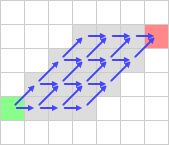
\includegraphics[width=0.4\textwidth]{figures/symmetricpath.png}\label{fig:symmetricpath}}
        \hfill
        \subfloat[Natural order of exploration in $JPS$.]{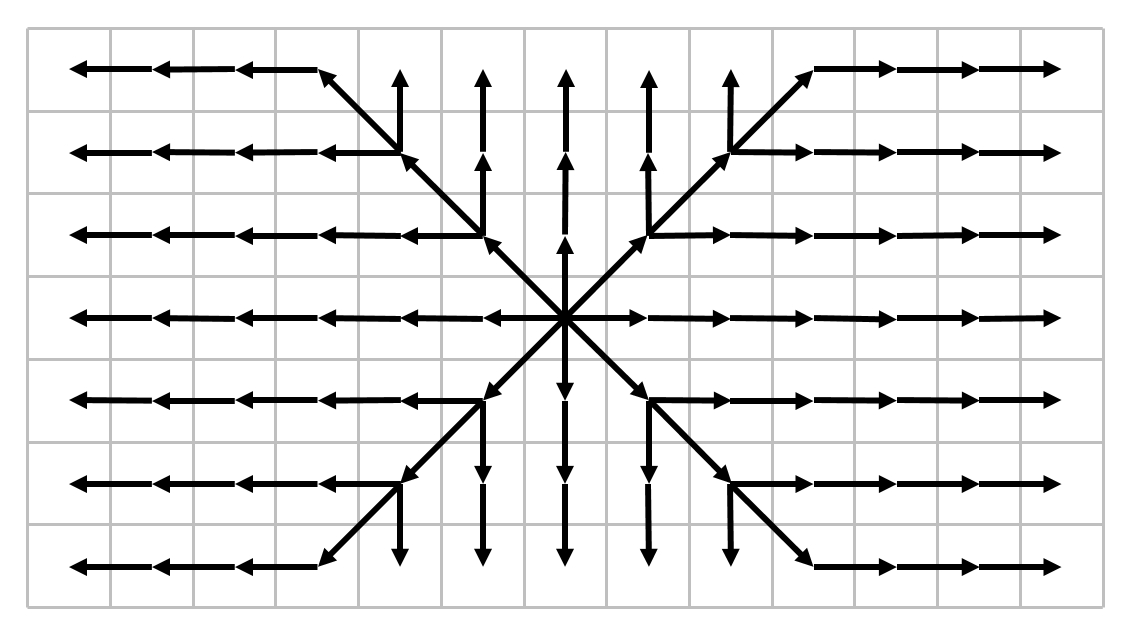
\includegraphics[width=0.4\textwidth]{figures/jps_strategy.png}\label{fig:pathorder}}
    \end{figure}
    

    To calculate the shortest path efficiently we can make use of the following observation. As long there are no changes in direction on the searched shortest path we can skip those points and jump to the last vertex before the direction change. Thus it seems to be efficient to find all points where the direction may change and adds only this specific points to the open list and ignores the others. In the figures group below is shown how to proceed to find these so called jump points. 
    
    The figures~\ref{fig:dm}~and~\ref{fig:dm_forced} show how to proceed with diagonal movements which are preferred over orthogonal movements. First of all we explore the orthogonal directions which are aligned to the diagonal movement. Whenever the algorithm finds a jump poin during exploration the outgoing point becomes a jump point and is added to the open list. If there is no jump point found, we skip the current point, add it not to the open list and continue at the next point in diagonal direction. In case of an passed obstacle the point right behind the obstacle will not be reached by any of the orthogonal explorations. Therefore this field becomes a forced field and the current explored field becomes a jump point and is added to the open list. Exploring in orthogonal directions is quiet similar. We jump over all points in the required orthogonal direction until we found out that there is nothing or until we pass an obstacle. In this case there is a forced field behind this obstacle which is not found by any preferred diagonal movement, because obstacle hinders movement. This makes the current point become a jump point and its added to the open list. 
    
    The colored points in the pictures have a special meaning. The green point is the currently being explored point. The grey points are points which are not visited because they are reached faster by the predecessor of the current point. The purple points are forced fields of the current point and black points are obstacles.
    
    
    
    
    \begin{figure}[!htb]
        \centering
        
        \caption{JPS exploring rules \cite{JPSexplained}.}
        
        \subfloat[diagonal moves.]{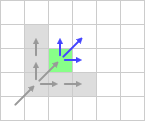
\includegraphics[width=0.4\textwidth]{figures/dm.png}\label{fig:dm}}
        \hfill
        \subfloat[diagonal moves with obstacle.]{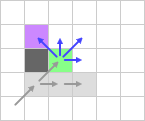
\includegraphics[width=0.4\textwidth]{figures/dm_forced.png}\label{fig:dm_forced}}
        
        \subfloat[orthogonal moves.]{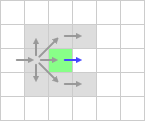
\includegraphics[width=0.4\textwidth]{figures/sm.png}\label{fig:sm}}
        \hfill
        \subfloat[orthogonal moves with obstacle.]{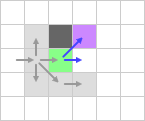
\includegraphics[width=0.4\textwidth]{figures/sm_forced.png}\label{fig:sm_forced}}
    \end{figure}
    
    Whenever a point is taken from the open list to explore all directions to forced fields, the orthogonal directions aligned to the diagonal direction and the current incoming direction are explored in this order.
    
    
    \subsection{Jump point search Improvements $JPS^+$}
    
    There is an improvement of $JPS$ called $JPS^+$~\cite{DBLP:conf/aips/HaraborG14}. Its a preprocessing technique to reduce the work of $JPS$ during runtime. The preprocessing is done by calculating for every passable point and every outgoing direction the next jump point on the map and stores this information in a look-up table together with the cost for that jump. During the search at runtime the algorithm just takes in every explore step the stored value from the lookup table and adds the costs instead of exploring the map.
    
        
    \begin{figure}[!htb]
        \centering
        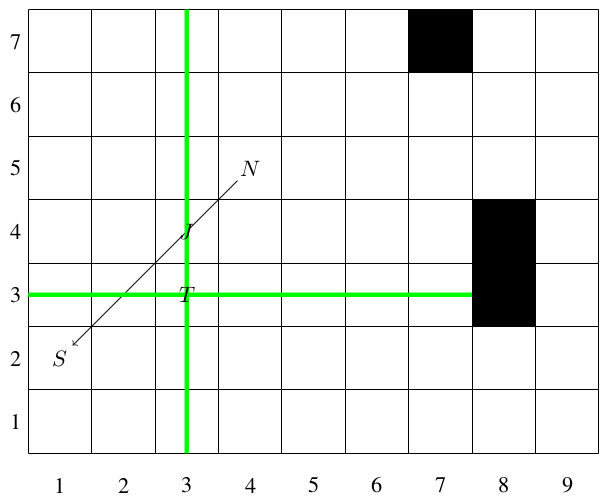
\includegraphics[width=\textwidth]{figures/jpspluspic.png}
        \caption{Goal point modification in $JPS^+$}
        \label{fig:jpsplus}
    \end{figure}
    
    
    The goal point is not necessarily a jump point, because the goal point is not known while preprocessing. That has to be taken into account. To do so we add jump points at runtime whenever jumping past the goal point. Figure~\ref{fig:jpsplus} is an example where we are at $N$ jumping to $S$ past goal point $T$. To avoid that we add $J$ as the next jump point to the open list to find $T$.


    
    
    \subsection{Bounding boxes pruning $BB$}
    
    Bounding boxes is a pruning technique that can be applied to lot of different path finding algorithms~\cite{DBLP:conf/aaai/RabinS16}. The pruning requires some preprocessing which can be done offline, i.e. before the actual start and goal point are known.
    
    For each pair of points and direction we have a dedicated bounding box. This box consists of all points which are can be reached optimally on a path from that given point. The box itself is the smallest geometric container, in this case a rectangle, to have every of those points inside. This implies that any point outside the box will be pruned since they will not help finding an optimal path.
    
    The bounding depends on the underlying algorithms, in case of $A^\star$ and $JPS$ it is sufficient to have minimum and maximum values for the X and Y coordinates. For $A^\star$ we can determine a predecessor $p$ for the point $v$ by inverting the direction. Then the bounding box of the point consists of all points which have a shortest path from $p$ to those points using $v$ as intermediate point. For $JPS$ we can go even further and use the knowledge of our jump points and natural ordering. Here the pruning will be even more effective which can be observed in our visualization of the algorithm.
    
    \begin{figure}[!htb]
        \centering
        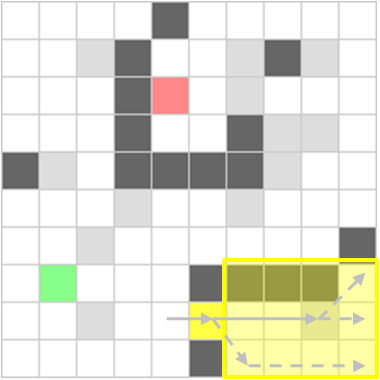
\includegraphics{figures/bounding_boxes.png}
        \caption{Visualization of bouding boxes.}
        \label{fig:bounding_boxes}
    \end{figure}
    
    
    
    
    \section{Implementation}
    
    \subsection{Application Core}
    
    The main goal and therefore the most important part of the lab work was to implement our algorithms. Our core offers an interface for external usage. One can use it as a library for any kind of application. We split up every choice of algorithm settings in a way everything can be combined as needed. The algorithm settings have the main point algorithmic structure, heuristic function and grid graph movement rules. The structure is the basis of everything, here you can choose between every algorithm described above. The algorithms are $A^\star$, $JPS$ and $JPS^+$. Everyone can be additionally combined with bounding boxes pruning to speed up search. The heuristic functions can be chosen from one of the commonly used ones which are Manhattan distance, Euclidean distance or Grid distance. Grid distance is the shortest possible distance on any grid graph where no obstacle hinders the movement. Its also possible to choose no heuristic function which will for example make $A^\star$ behave like the Dijkstra algorithm. At last one has to choose the movement rule. The decides in which way an algorithm is allowed to move on the grid graph. One option is orthogonal movement where every diagonal edge is forbidden. The other options decide whether edge cutting is allowed. Edge cutting offers an option to use diagonal edges even though part of an obstacle is lying on the way.
    
    
    \subsection{Visualization and user interface}
    
    The visualization is the second substantial aspect of our work. To begin we will explain the basic working of the user interface. At first one can use the \textit{File} menu to load any map. There are a number of different possibilities to create a random map satisfying a specific layout, for example perfect mazes or random rooms connected in a selected way. The next menu is \textit{Edit} where the user can edit the map or change the algorithm settings. We offer $A^\star$, $JPS$, $JPS^+$ and each of them with additional $BB$ pruning. Those algorithms are explained in section~\ref{sec:algorithms}. On top of that one can modify each of those algorithms by choosing a heuristic and a moving rule. The heuristic modification leads into situations where different candidates of the open list will be explored. The change in the moving rule offers interesting observations when used with some kinds of jump point search and shows also the limits of jump point search. Then the user is supposed to pick locations for the start and goal point. Then the algorithm can be run after some prepossessing if necessary. We have separate steps for those actions, so one can easily modify the algorithm settings and see the changes after running the other algorithm settings.
    
    The visualization will show the result of the algorithms. The red line between the chosen start and goal point indicates the shortest path. We have different colors for points which are in the open list or closed list. Every type of points can be shown or hidden by using the \textit{View} menu.
    
    The Java implementation is written using JavaFX, the successor of Swing.
    
    \begin{figure}[!htb]
        \centering
        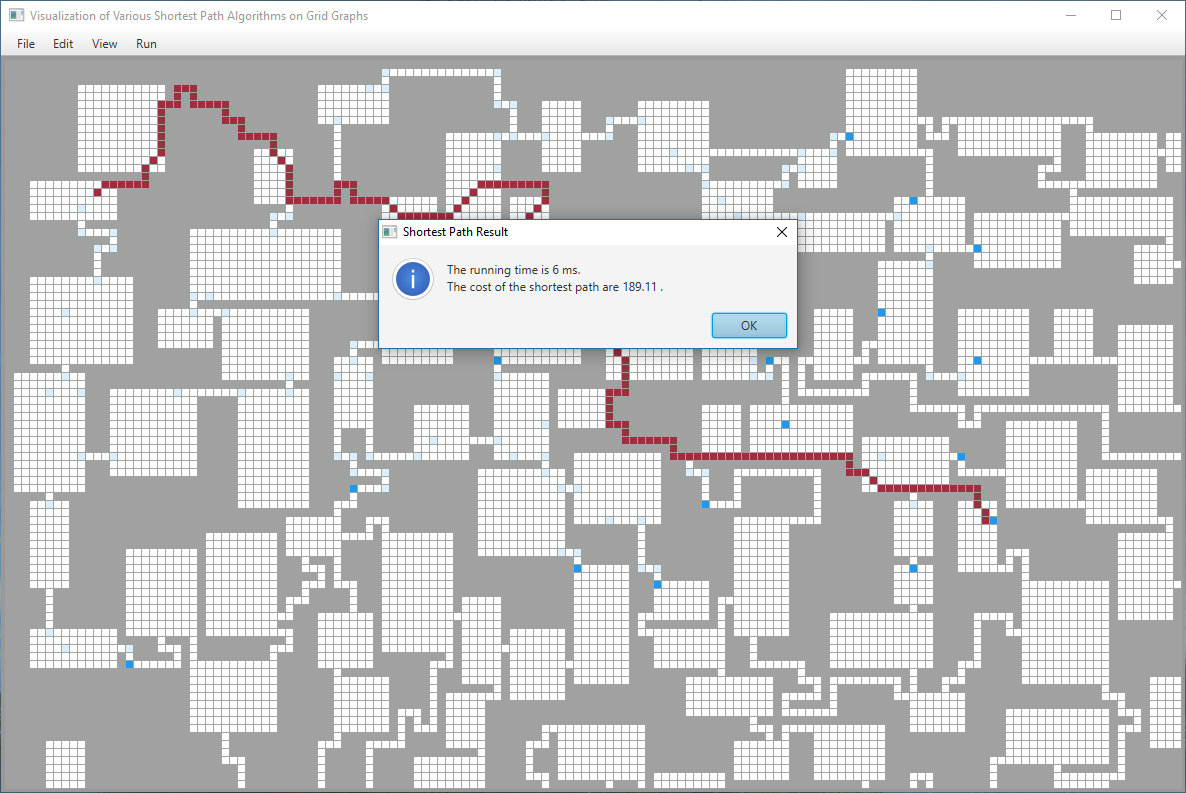
\includegraphics[width=\textwidth]{figures/javafx.png}
        \caption{Screenshot of the user interface.}
        \label{fig:javafx}
    \end{figure}
    
    
    
    \subsection{Benchmarking measurements}
    \label{sec:benchmarking}
    
    In addition to the visualization we wrote a benchmark application for terminal usage. This benchmark application could be used by other people who want to find out which algorithm settings is best for their real world application. We used it for a given set of benchmark maps and so called scenarios to find out how other our implementations are. The results of this benchmarking can be found in section~\ref{sec:results}. The usage of the terminal is simple. You can start it by using following command
    
    \begin{lstlisting}[basicstyle=\small\ttfamily]
      # java -classpath $PATH_TO_JAR$/LabApplication.jar
        terminalapplication.Main $DIR$ $ALGO$
    \end{lstlisting}
    
    In that command we have three parameters where the name should be self-explaining. The accepted names of algorithms are $astar$, $astarbb$, $jps$, $jpsbb$, $jpsplus$, $jpsplusbb$. The directory has some requirements to be fulfilled. The first is that a directory with that name is a sub directory in both \textit{maps} and \textit{scenarios} directory. In the sub directory in maps there has to be maps with .map suffix and format encoding as in MovingAI \cite{sturtevant2012benchmarks}. The same holds for the sub directory in scenarios, where each file has to have the .scen suffix and appropriate encoding.
    
    Each map will we processed along with the corresponding scenario file. To benchmark a single map it has to be in its own folder if that is necessary.
    
    
    
    \section{Results}
    \label{sec:results}
    
    This section presents the experiment results on the benchmark data from MovingAI lab.\cite{sturtevant2012benchmarks} The experiments were executed by our benchmark application described in section~\ref{sec:benchmarking}. The benchmarking data are divided into different map types which are artificial maps like mazes, rooms, random maps or real maps from existing computer games. For each type there exist between 40 and 160 of map instances with 5000 to 15000 pairs of start and goal points. A pair of start and goal point for measurement is referred to as scenario.
    
    Every map measurement that was executed by our application did match the same results as the original benchmarks. Therefore our algorithm implementations seem to be are correct and bug free holds. The plotting of our measurement data is built up into two steps. For all map scenarios the average value for the category (e.g. runtime) is calculated. The second step was to determine the whisker boxes of the resulting average values. This was done to avoid a weighting of maps, because different maps have a different number of scenarios.
    
    The first group of plots compares the runtime for searching a shortest path of different map types with different algorithms. $A^\star$ is performing very bad in every scenario when compared to any jump point search algorithm. In the figures~\ref{fig:00_time_mazes_sub}, \ref{fig:01_time_rooms_sub} and \ref{fig:02_time_random} is shown that $JPS^+$ does not perform better than $JPS$ and $BB$ have a significant influence on the runtime on artificial map types. In contrast to the artificial maps we have the plots of real maps in figures\ref{fig:03_time_bg512}, \ref{fig:04_time_da2} and \ref{fig:05_time_sc1}. Here the influence of $JPS^+$ dominates the influence of $BB$. This seems logical since real maps include big areas of passable fields which have to be explored while executing $JPS$ while exploring these big areas are done in preprocessing in the $JPS^+$ setting. In consequence $JPS^+$ makes just one big step while passing these areas while $JPS$ explores them completely in runtime. Moreover figure~\ref{fig:03_time_bg512} shows that bounding boxes can have a bad influence on the runtime, especially observable for on $A^\star$ and on $A^\star + BB$. Bounding boxes require additional time for each step to decide whether an expansion node can be ignored. If the pruning can be applied too seldom, then the cost for the bounding boxes check ups might be more expensive than the gain of exploring less points.
    
    In figures~\ref{fig:06_mazes_normalscale}~and~\ref{fig:07_mazes_logscale} we compare different sized mazes where the size is the width of a floor in the maze. The result plot supports the observation made in the previous plots. The bigger the floors are, the more the results come close the real world maps. $A^\star$ performs the worse the bigger the floor size is. Meanwhile $JPS^+$ performs even better during a growing size. With growing floor size (resulting in more connected passable space) the influence of the different exploring algorithms dominates the effect of bounding boxes.
    
    Figures~\ref{fig:preprocessing_mazes_sub},~\ref{fig:08_preprocessing_bg512}~and~\ref{fig:preprocessing_da2} show that the preprocessing time for bouding boxes in independent of the underlying algorithm. This comes from the fact that the most part of the computation is the same in every case. $JPS^+$ is incredible fast and is completed in milliseconds even though bounding boxes may need several hours. Figure~\ref{fig:09_preprocessing_jpsplusbb} shows that the preprocessing effort for bounding boxes in artificial maps is significant bigger than in real maps. That is because artificial maps have much more passable fields and calculation requires to explore the whole map for every passable field. The total effort therefore is $\Omega(m^2)$ where $m$ is the amout of passable fields on the map.
    
    \begin{figure}[!htb]
        \centering
        
        \caption{Runtime to find the shortest path.}
        
        
        \subfloat[Runtime in mazes.]{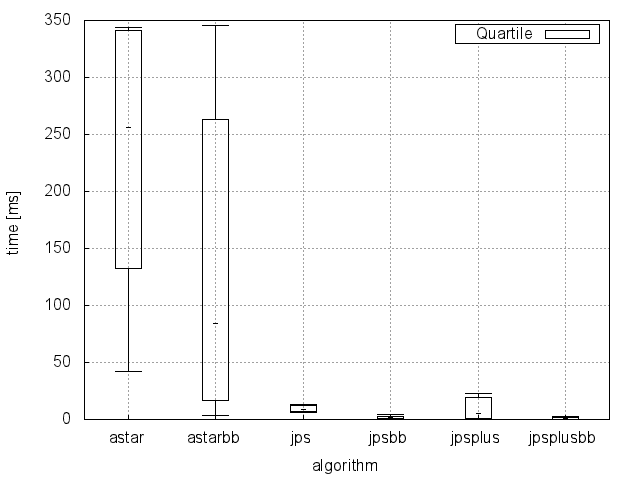
\includegraphics[width=0.49\textwidth]{figures/00_time_mazes_sub.png}\label{fig:00_time_mazes_sub}}
        \hfill
        \subfloat[Runtime in rooms.]{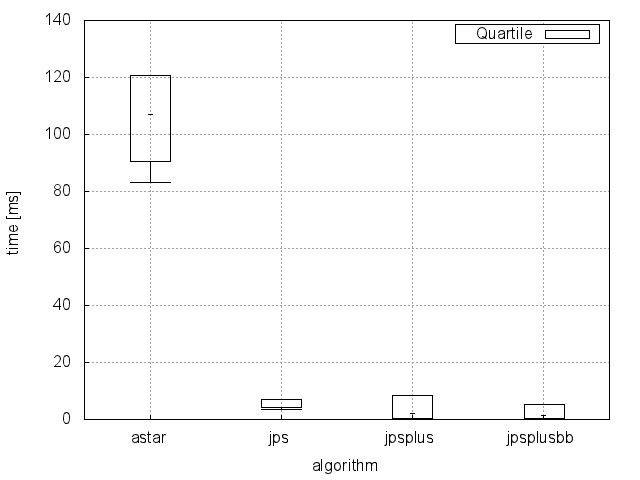
\includegraphics[width=0.49\textwidth]{figures/01_time_rooms_sub.png}\label{fig:01_time_rooms_sub}}
        
        \subfloat[Runtime on random maps.]{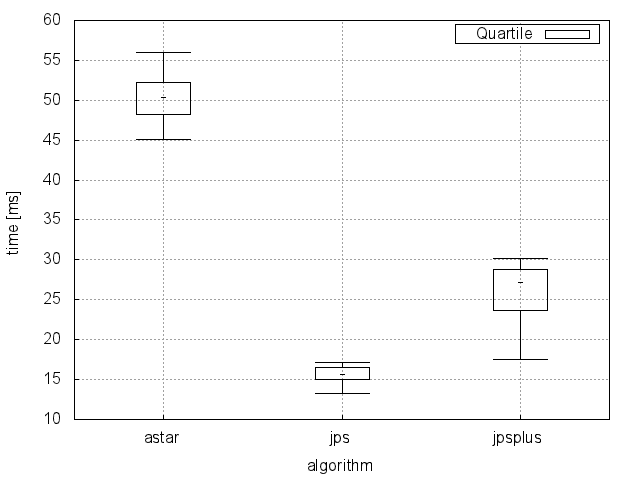
\includegraphics[width=0.49\textwidth]{figures/02_time_random.png}\label{fig:02_time_random}}
        \hfill
        \subfloat[Runtime on Baldurs Gate maps.]{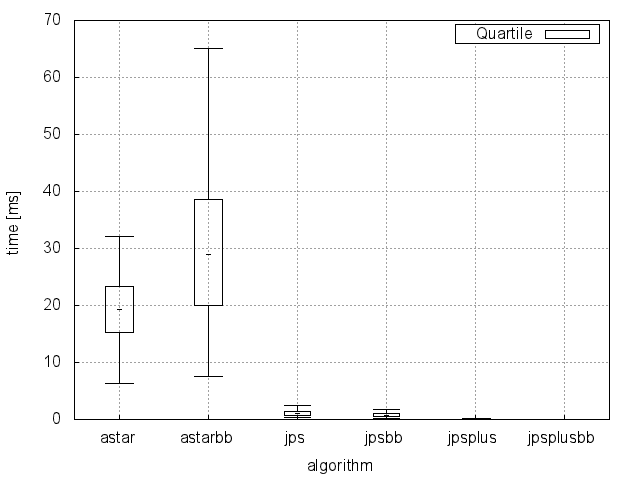
\includegraphics[width=0.49\textwidth]{figures/03_time_bg512.png}\label{fig:03_time_bg512}}
        
        \subfloat[Runtime on Dragon Age maps.]{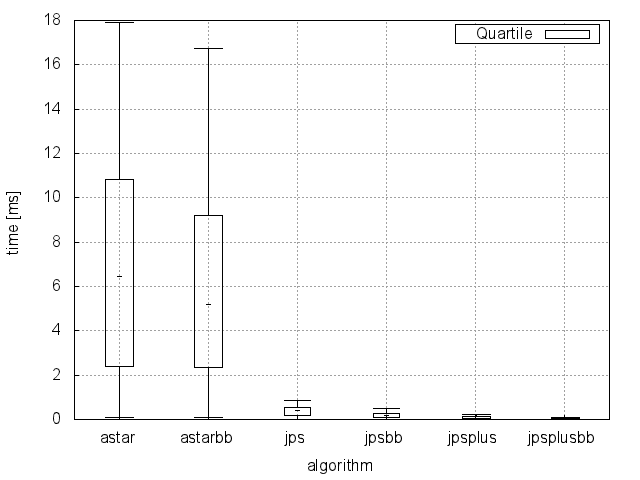
\includegraphics[width=0.49\textwidth]{figures/04_time_da2.png}\label{fig:04_time_da2}}
        \hfill
        \subfloat[Runtime on StarCraft maps.]{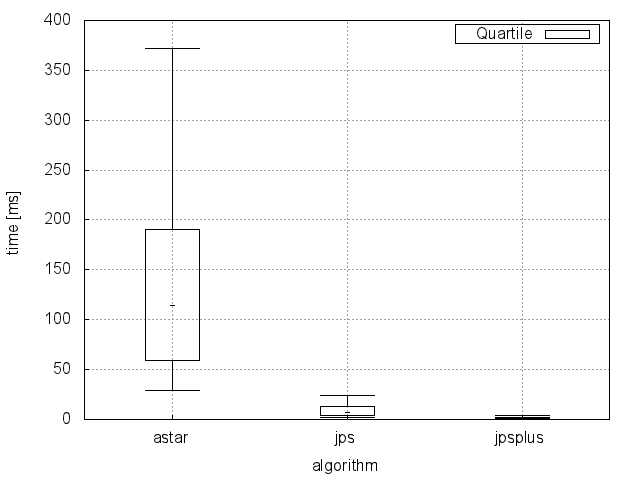
\includegraphics[width=0.49\textwidth]{figures/05_time_sc1.png}\label{fig:05_time_sc1}}
        
    \end{figure}
    
    \begin{figure}[!htb]
        \centering
        
        \caption{Runtime to find the shortest path in different mazes.}
        
        \subfloat[Runtime in different sized mazes.]{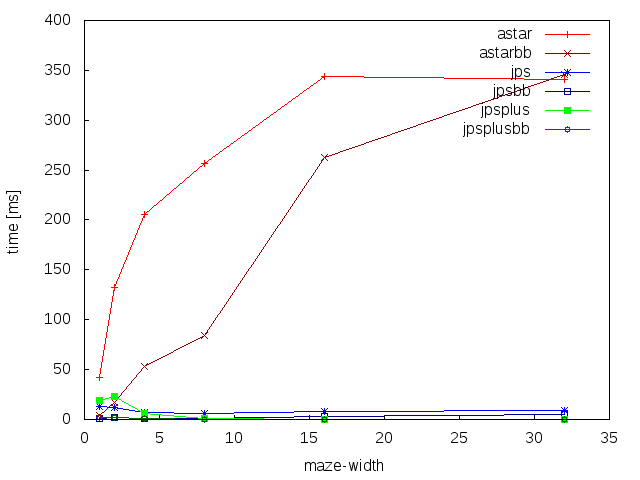
\includegraphics[width=0.49\textwidth]{figures/06_mazes_normalscale.png}\label{fig:06_mazes_normalscale}}
        \hfill
        \subfloat[Runtime in different sized mazes with logscale.]{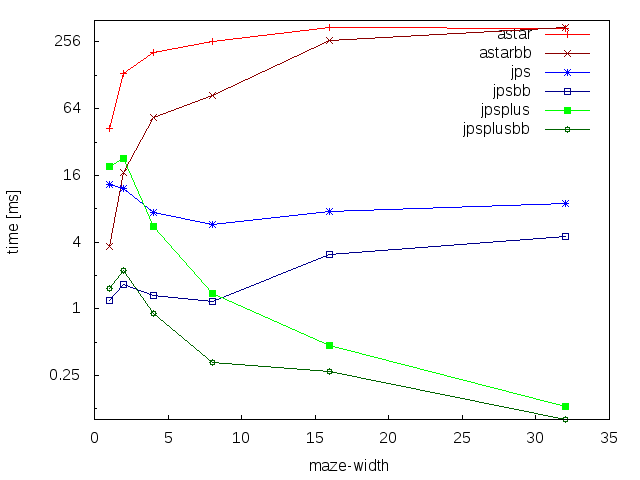
\includegraphics[width=0.49\textwidth]{figures/07_mazes_logscale.png}\label{fig:07_mazes_logscale}}
    \end{figure}
    
    \begin{figure}[!htb]
        \centering
        
        \caption{Preprocessing time to find the shortest path.}
        
        \subfloat[Preprocessing time in mazes.]{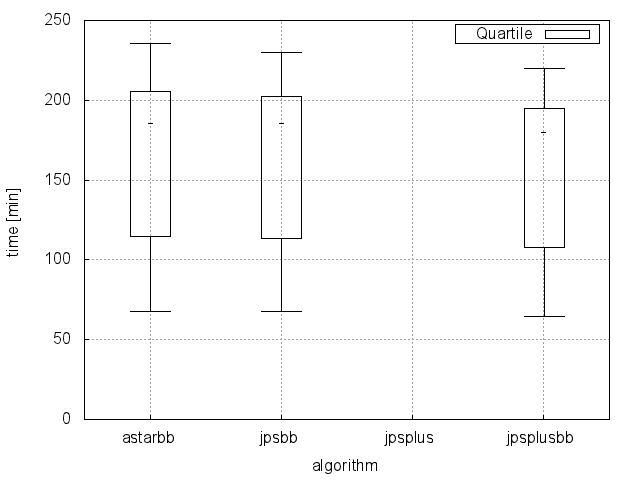
\includegraphics[width=0.49\textwidth]{figures/preprocessing_mazes_sub.png}\label{fig:preprocessing_mazes_sub}}
        \hfill
        \subfloat[Preprocessing time on Baldurs Gate maps.]{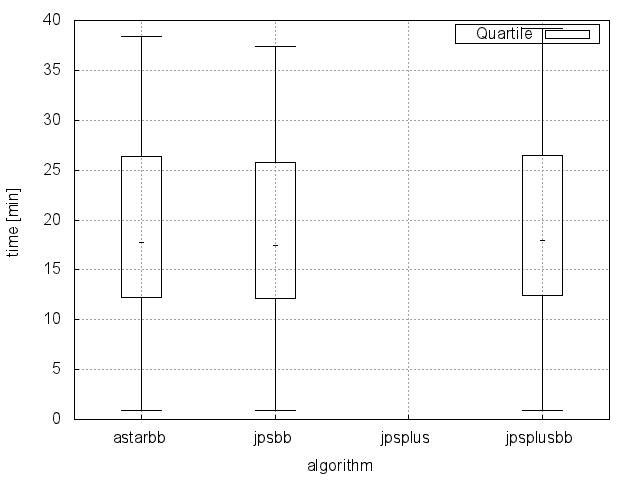
\includegraphics[width=0.49\textwidth]{figures/08_preprocessing_bg512.png}\label{fig:08_preprocessing_bg512}}
        
        \subfloat[Preprocessing time on Dragon Age maps.]{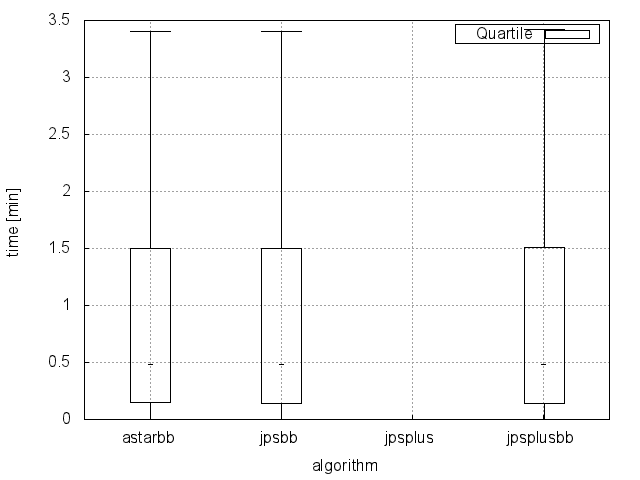
\includegraphics[width=0.49\textwidth]{figures/preprocessing_da2.png}\label{fig:preprocessing_da2}}
        \hfill
        \subfloat[Preprocessing time for JPS+ with BB on different map types.]{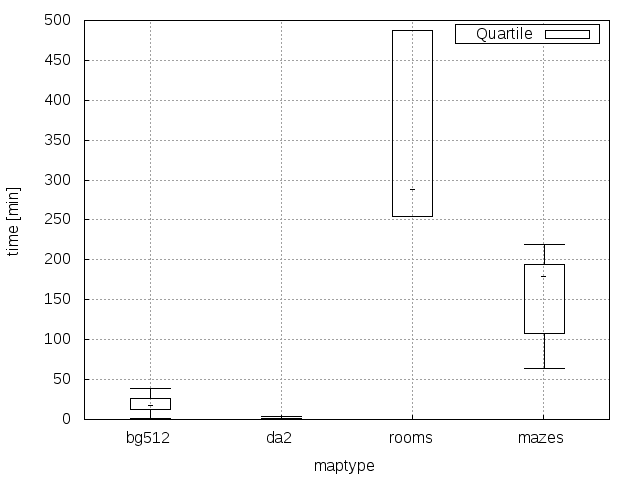
\includegraphics[width=0.49\textwidth]{figures/09_preprocessing_jpsplusbb.png}\label{fig:09_preprocessing_jpsplusbb}}
    \end{figure}
 
    
    
    
    
    \bibliographystyle{alpha}
    \bibliography{references}
\end{document}
